\documentclass[10pt,a4paper]{article}
\usepackage{tocloft}
\usepackage{commons/course}  % همین کافیه؛ listings و xcolor داخلشه
\usepackage{booktabs}
\usepackage{longtable}
\usepackage{float}

\definecolor{keywordstyle}{rgb}{0.0, 0.4, 0.8}
\definecolor{stringstyle}{rgb}{0.9, 0.17, 0.31}
\definecolor{commentstyle}{rgb}{0.1, 0.6, 0.2}
\definecolor{numberstyle}{rgb}{0.4, 0.4, 0.4}
\definecolor{backgroundcolor}{rgb}{0.94, 0.97, 1.0}

\lstdefinelanguage{PythonLike}{
	morekeywords={mov, add, sub, cmp, jmp , lw , addi,sw,bne},
	sensitive=false,
	morecomment=[l]{;},
	morestring=[b]",
}

\lstset{
	language=PythonLike,
	basicstyle=\ttfamily\small,
	keywordstyle=\color{keywordstyle},
	stringstyle=\color{stringstyle},
	commentstyle=\color{commentstyle},
	numbers=left,
	numberstyle=\tiny\color{numberstyle},
	stepnumber=1,
	numbersep=5pt,
	keepspaces=true,
	tabsize=4,
	showspaces=false,
	showstringspaces=false,
	showtabs=false,
	breaklines=true,
	breakatwhitespace=false,
	frame=single,
	backgroundcolor=\color{backgroundcolor},
}

\newlistof{listofproblems}{lop}{\normalsize فهرست مسائل}
\newcommand{\addproblem}[1]{\addcontentsline{lop}{listofproblems}{\protect\numberline{}#1}}


\begin{document}


\سربرگ{آزمایش ششم}{واحد محاسبه با انتخاب ثبات مبدا و مقصد}{معین آعلی - ثمین اکبری}{استاد: دکتر حمید سربازی آزاد}

\subsubsection*{خلاصه}

در این آزمایش واحد محاسبات و مجموعه ثبات‌های عمومی ماشین طراحی و پیاده‌سازی شده است. مدار چهار ثبات عمومی هشت‌بیتی \lr{R0} تا \lr{R3} دارد و می‌تواند جمع و تفریق را با انتخاب ثبات مبدا و ثبات مقصد انجام دهد. یکی از عملوندهای \lr{ALU} همیشه محتوای \lr{R0} است و عملوند دیگر یکی از چهار ثبات یا یکی از مقادیر ثابت ۰، ۱ و ۱− است. مدار فرمان‌های شش بیتی مشخص‌شده در دستور کار را اجرا می‌کند.



\begin{figure}[H]
  \centering
  
\includegraphics[width=0.8\textwidth]{figs/block.png}
\end{figure}


\subsubsection*{هدف آزمایش}

طی آزمایش‌های ششم، هفتم و هشتم یک کامپیوتر ساده به‌طور کامل طراحی و پیاده‌سازی می‌شود و برنامه‌ای به زبان ماشین روی آن اجرا می‌گردد. این آزمایش اولین گام آن مسیر است. اهداف مشخص عبارت‌اند از:

\begin{itemize}
  \item طراحی مجموعه ثبات‌های عمومی با قابلیت انتخاب ثبات مبدا و مقصد.
  \item پیاده‌سازی واحد محاسباتی با قابلیت جمع و تفریق.
  \item آشنایی با قالب فرمان و رمزگشایی میدان‌های آن.
  \item بررسی صحت عملکرد با اجرای تمام فرمان‌های ممکن.
\end{itemize}


\subsubsection*{قالب فرمان}

فرمان‌ها شش بیتی‌اند و از سه میدان تشکیل شده‌اند:

\begin{center}
\begin{tabular}{@{}cccccc@{}}
\toprule
\lr{bit 5} & \lr{bit 4} & \lr{bit 3} & \lr{bit 2} & \lr{bit 1} & \lr{bit 0} \\
\midrule
\lr{F} & \multicolumn{2}{c}{\lr{D1 \quad D0}} & \multicolumn{3}{c}{\lr{S2 \quad S1 \quad S0}} \\
\lr{ALU function} & \multicolumn{2}{c}{\lr{Destination}} & \multicolumn{3}{c}{\lr{Source}} \\
\bottomrule
\end{tabular}
\end{center}

\begin{center}
\begin{tabular}{@{}lll@{}}
\toprule
{میدان} & {مقدار} & {معنی} \\
\midrule
\lr{F} & \lr{0} & جمع \\
       & \lr{1} & تفریق \\
\midrule
\lr{D} & \lr{00} تا \lr{11} & ثبات مقصد \lr{R0} تا \lr{R3} \\
\midrule
\lr{S} & \lr{000} تا \lr{011} & ثبات مبدا \lr{R0} تا \lr{R3} \\
       & \lr{100} & مقدار ثابت ۰ \\
       & \lr{101} & مقدار ثابت ۱ \\
       & \lr{110} & مقدار ثابت ۱− \\
       & \lr{111} & رزرو برای جلسه‌ی بعد \\
\bottomrule
\end{tabular}
\end{center}

عملی که در هر فرمان انجام می‌شود همیشه به این شکل است:
\[
R_d \;\leftarrow\; R_0 \;(+ \text{ یا } -)\; \mathrm{src}
\]

یعنی یک عملوند همیشه \lr{R0} است. با این قالب $2 \times 4 \times 7 = 56$ فرمان معتبر وجود دارد (میدان مبدا \lr{111} رزرو است).

مقدار ثابت ۱− در متمم دو هشت‌بیتی برابر \lr{0xFF} است، بنابراین $R_0 + (-1)$ دقیقا همان $R_0 - 1$ می‌شود؛ این هم‌ارزی برای تمام ۲۵۶ مقدار ممکن بررسی و تأیید شد.

\vspace{0.5em}
دو نمونه فرمان:

\begin{center}
\begin{tabular}{@{}llll@{}}
\toprule
{فرمان} & {باینری} & {میدان‌ها} & {عمل} \\
\midrule
\lr{0x0D} & \lr{001101} & \lr{F=0, D=01, S=101} & $R_1 \leftarrow R_0 + 1$ \\
\lr{0x31} & \lr{110001} & \lr{F=1, D=10, S=001} & $R_2 \leftarrow R_0 - R_1$ \\
\bottomrule
\end{tabular}
\end{center}


\subsubsection*{رابط مدار}

مدار اصلی \lr{datapath} است و مدار \lr{main} همان را با یک قطعه‌ی \lr{Clock} و ورودی‌های مجزا برای نمایش می‌پیچد.

\begin{center}
\begin{tabular}{@{}llll@{}}
\toprule
{سیگنال} & {جهت} & {پهنا} & {توضیح} \\
\midrule
\lr{IR} & ورودی & ۶ & فرمان \\
\lr{WE} & ورودی & ۱ & فعال‌ساز نوشتن؛ با ۰ هیچ ثباتی تغییر نمی‌کند \\
\lr{clk} & ورودی & ۱ & لبه‌ی بالارونده؛ هر لبه یک فرمان اجرا می‌کند \\
\lr{rst} & ورودی & ۱ & پاک‌سازی آسنکرون همه‌ی ثبات‌ها \\
\lr{R0}--\lr{R3} & خروجی & ۸ & محتوای ثبات‌های عمومی \\
\lr{ALUout} & خروجی & ۸ & خروجی \lr{ALU} (برای مشاهده) \\
\lr{Cout} & خروجی & ۱ & رقم نقلی خروجی (برای مشاهده) \\
\bottomrule
\end{tabular}
\end{center}

سیگنال \lr{WE} در دستور کار نیامده ولی برای تک‌گام‌کردن و توقف مدار لازم است؛ در آزمایش‌های بعدی که واحد کنترل اضافه می‌شود همین سیگنال از واحد کنترل خواهد آمد.


\subsubsection*{معماری مدار}

جریان داده در هر فرمان چنین است: میدان \lr{S} یکی از هشت ورودی مالتی‌پلکسر را انتخاب می‌کند؛ خروجی مالتی‌پلکسر از آرایه‌ی گیت‌های \lr{XOR} می‌گذرد تا در صورت تفریق متمم شود؛ جمع‌کننده آن را با \lr{R0} جمع می‌کند؛ و نتیجه روی ورودی هر چهار ثبات می‌نشیند، ولی فقط ثباتی که رمزگشا انتخابش کرده در لبه‌ی ساعت آن را می‌پذیرد.

\begin{center}
\begin{tabular}{@{}lll@{}}
\toprule
{قطعه} & {تعداد} & {نقش} \\
\midrule
\lr{Adder} (۸ بیتی) & ۱ & جمع و تفریق \\
\lr{Multiplexer} (۸ به ۱) & ۱ & انتخاب عملوند مبدا \\
\lr{Register} (۸ بیتی) & ۴ & ثبات‌های عمومی \lr{R0} تا \lr{R3} \\
\lr{XOR Gate} & ۸ & متمم‌کردن عملوند دوم هنگام تفریق \\
\lr{XOR Gate} & ۲ & ساخت مکمل بیت‌های مقصد \\
\lr{AND Gate} (۳ ورودی) & ۴ & رمزگشای مقصد \\
\lr{Constant} & ۵ & مقادیر ثابت ۰، ۱، ۱− و \lr{VCC}/\lr{GND} \\
\lr{Splitter} & ۴ & جداکردن میدان‌های فرمان و بیت‌های باس \\
\bottomrule
\end{tabular}
\end{center}


\subsubsection*{نکته‌ی اول: جمع و تفریق با یک جمع‌کننده}

به‌جای ساختن مدار تفریق جداگانه، از خاصیت متمم دو استفاده شده است:
\[
A - B \;=\; A + \overline{B} + 1
\]

بنابراین اگر هر بیت عملوند دوم را با بیت تابع \lr{F} گیت \lr{XOR} کنیم و خود \lr{F} را هم به ورودی رقم نقلی جمع‌کننده بدهیم:

\[
\begin{aligned}
F = 0 &:\quad R_0 + \mathrm{src} + 0 &&= R_0 + \mathrm{src} \\
F = 1 &:\quad R_0 + \overline{\mathrm{src}} + 1 &&= R_0 - \mathrm{src}
\end{aligned}
\]

چون $x \oplus 0 = x$ و $x \oplus 1 = \bar{x}$، همان یک سیگنال \lr{F} هم متمم‌کردن را کنترل می‌کند و هم رقم نقلی ورودی را تأمین می‌کند. هزینه‌ی این کار فقط هشت گیت \lr{XOR} است و {یک جمع‌کننده هر دو عمل را انجام می‌دهد}.


\subsubsection*{نکته‌ی دوم: رمزگشای مقصد}

هر چهار ثبات خروجی \lr{ALU} را روی ورودی \lr{D} و ساعت مشترک می‌بینند. تفاوت‌شان فقط در پایه‌ی \lr{en} است:

\[
\mathrm{EN}_k \;=\; \mathrm{WE} \cdot (D_1 = k_1) \cdot (D_0 = k_0)
\]

یعنی برای هر ثبات یک گیت \lr{AND} سه‌ورودی لازم است که ترکیب درست بیت‌های مقصد را تشخیص دهد:

\begin{center}
\begin{tabular}{@{}llll@{}}
\toprule
{ثبات} & {مقدار} \lr{D} & {ورودی‌های گیت} & {خروجی} \\
\midrule
\lr{R0} & \lr{00} & \lr{WE}, \lr{nD1}, \lr{nD0} & \lr{EN0} \\
\lr{R1} & \lr{01} & \lr{WE}, \lr{nD1}, \lr{D0} & \lr{EN1} \\
\lr{R2} & \lr{10} & \lr{WE}, \lr{D1}, \lr{nD0} & \lr{EN2} \\
\lr{R3} & \lr{11} & \lr{WE}, \lr{D1}, \lr{D0} & \lr{EN3} \\
\bottomrule
\end{tabular}
\end{center}

چون \lr{WE} در هر چهار گیت هست، با $\mathrm{WE}=0$ تمام فعال‌سازها صفر می‌شوند و هیچ ثباتی تغییر نمی‌کند.

مکمل بیت‌های مقصد با $\mathrm{XOR}(x, 1)$ ساخته شده و نه با گیت \lr{NOT}. علت این است که در آزمایش دوم مشخص شد گیت \lr{NOT} تولیدشده در فایل گاهی بی‌صدا حذف می‌شود و هیچ خطایی هم چاپ نمی‌گردد؛ استفاده از \lr{XOR} با ورودی ثابت یک این مشکل را ندارد.

{نکته‌ی مهم درباره‌ی مقصد و مبدا یکسان.} چون ثبات‌ها لبه‌ای (\lr{edge-triggered}) هستند، وقتی مقصد و مبدا یکی باشند — مثلا فرمان $R_0 \leftarrow R_0 + R_0$ — مقدار {قبلی} ثبات خوانده می‌شود و نتیجه درست است. اگر ثبات‌ها سطحی بودند این حالت حلقه‌ی ترکیبی می‌ساخت. این حالت جداگانه تست شده است.


\subsubsection*{جزئیات پایه‌های قطعات}
در این بخش برای هر قطعه، نام پایه و سیگنالی که به آن وصل شده آورده شده است. این جدول‌ها مستقیم از فایل مدار تولید شده‌اند، پس دقیقا همان چیزی‌اند که در مدار سیم‌کشی شده است.

\paragraph{جمع‌کننده‌ی هشت‌بیتی (واحد محاسبات)}\mbox{}\\
عملوند اول همیشه \lr{R0} است. عملوند دوم از آرایه‌ی \lr{XOR} می‌آید و رقم نقلی ورودی همان بیت تابع است، پس تفریق بدون مدار جداگانه انجام می‌شود.

\begin{center}
\small
\begin{tabular}{@{}lll@{}}
\toprule
{پایه} & {سیگنال} & {توضیح} \\
\midrule
\lr{A} & \lr{R0Q} & عملوند اول — محتوای ثبات R0 \\
\lr{B} & \lr{BX} & عملوند دوم — عملوند دوم بعد از متمم‌شدن \\
\lr{Cin} & \lr{F} & رقم نقلی ورودی — بیت تابع (۰ جمع، ۱ تفریق) \\
\lr{S} & \lr{RES} & حاصل جمع — نتیجه‌ی ALU \\
\lr{Cout} & \lr{COUT} & رقم نقلی خروجی — رقم نقلی خروجی \\
\bottomrule
\end{tabular}
\end{center}

\paragraph{ثبات‌های عمومی}\mbox{}\\
هر چهار ثبات یکسان سیم‌کشی شده‌اند: همه نتیجه‌ی \lr{ALU} را روی ورودی داده و ساعت مشترک می‌بینند و تنها در پایه‌ی فعال‌ساز با هم فرق دارند. پایه‌ی \lr{rst} همه به سیگنال پاک‌سازی وصل است.

\begin{center}
\small
\begin{tabular}{@{}lllll@{}}
\toprule
{پایه} & \lr{R0} & \lr{R1} & \lr{R2} & \lr{R3} \\
\midrule
\lr{D} & \lr{RES} & \lr{RES} & \lr{RES} & \lr{RES} \\
\lr{en} & \lr{EN0} & \lr{EN1} & \lr{EN2} & \lr{EN3} \\
\lr{clk} & \lr{CLK} & \lr{CLK} & \lr{CLK} & \lr{CLK} \\
\lr{rst} & \lr{RST} & \lr{RST} & \lr{RST} & \lr{RST} \\
\lr{Q} & \lr{R0Q} & \lr{R1Q} & \lr{R2Q} & \lr{R3Q} \\
\bottomrule
\end{tabular}
\end{center}

پایه‌ی \lr{D} همه‌ی ثبات‌ها به \lr{RES} یعنی نتیجه‌ی جمع‌کننده وصل است و پایه‌ی \lr{Q} هر ثبات مقدار خودش را به مالتی‌پلکسر و خروجی مدار می‌برد. \lr{Q} ثبات \lr{R0} علاوه بر این، عملوند اول جمع‌کننده را هم تأمین می‌کند.

\paragraph{مالتی‌پلکسر انتخاب مبدا}\mbox{}\\
مالتی‌پلکسر ۸ به ۱ و هشت بیت پهنا دارد. ورودی ۷ طبق دستور کار برای جلسه‌ی بعد رزرو است و برای اینکه شناور نماند به مقدار ثابت صفر بسته شده است.

\begin{center}
\small
\begin{tabular}{@{}lll@{}}
\toprule
{پایه} & {سیگنال} & {توضیح} \\
\midrule
\lr{in0} & \lr{R0Q} & ورودی 0 (کد مبدا \lr{000}) \\
\lr{in1} & \lr{R1Q} & ورودی 1 (کد مبدا \lr{001}) \\
\lr{in2} & \lr{R2Q} & ورودی 2 (کد مبدا \lr{010}) \\
\lr{in3} & \lr{R3Q} & ورودی 3 (کد مبدا \lr{011}) \\
\lr{in4} & \lr{K0} & ورودی 4 (کد مبدا \lr{100}) \\
\lr{in5} & \lr{K1} & ورودی 5 (کد مبدا \lr{101}) \\
\lr{in6} & \lr{KM1} & ورودی 6 (کد مبدا \lr{110}) \\
\lr{in7} & \lr{K0} & ورودی 7 (کد مبدا \lr{111}) — رزرو \\
\lr{sel} & \lr{SRC} & خطوط انتخاب \\
\lr{out} & \lr{SRCV} & خروجی \\
\bottomrule
\end{tabular}
\end{center}

\paragraph{رمزگشای مقصد}\mbox{}\\
چهار گیت \lr{AND} سه‌ورودی، هرکدام فعال‌ساز یک ثبات را می‌سازند. دو گیت \lr{XOR} هم مکمل بیت‌های مقصد را تولید می‌کنند.

\begin{center}
\small
\begin{tabular}{@{}lll@{}}
\toprule
{گیت} & {ورودی‌ها} & {خروجی} \\
\midrule
\lr{AND} & \lr{WE, nD1, nD0} & \lr{EN0} \\
\lr{AND} & \lr{WE, nD1, D0} & \lr{EN1} \\
\lr{AND} & \lr{WE, D1, nD0} & \lr{EN2} \\
\lr{AND} & \lr{WE, D1, D0} & \lr{EN3} \\
\lr{XOR} & \lr{D1, VCC} & \lr{nD1} \\
\lr{XOR} & \lr{D0, VCC} & \lr{nD0} \\
\bottomrule
\end{tabular}
\end{center}

هشت گیت \lr{XOR} دیگر هم عملوند دوم را بیت‌به‌بیت با \lr{F} ترکیب می‌کنند؛ ورودی اولشان از اسپلیتر مقدار مبدا می‌آید و خروجی‌شان با اسپلیتر دوم دوباره به یک باس هشت‌بیتی تبدیل می‌شود.


\subsubsection*{سیگنال‌های داخلی}

\begin{center}
\begin{tabular}{@{}lll@{}}
\toprule
{سیگنال} & {پهنا} & {معنی} \\
\midrule
\lr{F} & ۱ & بیت تابع: ۰ جمع، ۱ تفریق \\
\lr{DST} & ۲ & میدان مقصد فرمان \\
\lr{SRC} & ۳ & میدان مبدا فرمان \\
\lr{SRCV} & ۸ & مقدار عملوند مبدا (خروجی مالتی‌پلکسر) \\
\lr{BX} & ۸ & عملوند دوم پس از متمم‌شدن با \lr{F} \\
\lr{RES} & ۸ & نتیجه‌ی جمع‌کننده \\
\lr{R0Q}--\lr{R3Q} & ۸ & محتوای ثبات‌ها \\
\lr{D0}, \lr{D1} & ۱ & بیت‌های مقصد \\
\lr{nD0}, \lr{nD1} & ۱ & مکمل بیت‌های مقصد \\
\lr{EN0}--\lr{EN3} & ۱ & فعال‌ساز بارگذاری هر ثبات \\
\lr{K0}, \lr{K1}, \lr{KM1} & ۸ & مقادیر ثابت ۰، ۱ و ۱− \\
\bottomrule
\end{tabular}
\end{center}

مسیر داده از فرمان تا ثبات مقصد:
\[
\mathrm{SRC} \rightarrow \mathrm{SRCV} \xrightarrow{\;\oplus F\;} \mathrm{BX}
\xrightarrow{\;+R_0\;} \mathrm{RES} \xrightarrow{\;\mathrm{EN}_k\;} R_k
\]


\subsubsection*{نحوه‌ی استفاده}

\begin{enumerate}
  \item سیگنال \lr{rst} را یک لحظه ۱ کن تا همه‌ی ثبات‌ها صفر شوند.
  \item فرمان را روی \lr{IR} بگذار. در مدار \lr{main} سه میدان \lr{F}، \lr{DST} و \lr{SRC} جداگانه وارد می‌شوند و خود مدار آن‌ها را به فرمان شش بیتی تبدیل می‌کند.
  \item سیگنال \lr{WE} را ۱ کن.
  \item یک لبه‌ی ساعت بده. فرمان اجرا می‌شود و نتیجه در ثبات مقصد می‌نشیند.
\end{enumerate}

هر لبه‌ی ساعت دقیقا یک فرمان اجرا می‌کند. با $\mathrm{WE}=0$ هیچ ثباتی تغییر نمی‌کند، که برای تک‌گام‌کردن یا توقف مدار مفید است. در مدار \lr{main} یک قطعه‌ی \lr{Clock} واقعی هست که با \lr{Ctrl+K} تیک می‌خورد.

\vspace{0.5em}
نمونه‌ی اجرای یک برنامه‌ی کوتاه، با فرض اینکه از حالت صفر شروع کنیم:

\begin{RTL}
\begin{center}
\begin{tabular}{@{}cllcccc@{}}
\toprule
\lr{step} & \lr{instruction} & \lr{meaning} & \lr{R0} & \lr{R1} & \lr{R2} & \lr{R3} \\
\midrule
0 & (reset)  & --                     & 0 & 0 & 0 & 0 \\
1 & \lr{001101} & $R_1 \leftarrow R_0 + 1$   & 0 & 1 & 0 & 0 \\
2 & \lr{000101} & $R_0 \leftarrow R_0 + 1$   & 1 & 1 & 0 & 0 \\
3 & \lr{000101} & $R_0 \leftarrow R_0 + 1$   & 2 & 1 & 0 & 0 \\
4 & \lr{010001} & $R_2 \leftarrow R_0 + R_1$ & 2 & 1 & 3 & 0 \\
5 & \lr{111001} & $R_3 \leftarrow R_0 - R_1$ & 2 & 1 & 3 & 1 \\
\bottomrule
\end{tabular}
\end{center}
\end{RTL}


\subsubsection*{تست و صحت‌سنجی}

صحت مدار با بردارهای تست ترتیبی بررسی شده است. بردارها ستون‌های \lr{<Set>} و \lr{<Seq>} دارند: \lr{Logisim} در شروع هر \lr{<Set>} مدار را ریست می‌کند و بین گام‌های \lr{<Seq>} وضعیت را نگه می‌دارد.

\begin{center}
\begin{tabular}{@{}llr@{}}
\toprule
{فایل} & {مدار} & {پوشش} \\
\midrule
\lr{tests\_datapath.vec} & \lr{datapath} & سناریوهای هدفمند، ۲۹۸ گام \\
\lr{tests\_datapath\_random.vec} & \lr{datapath} & ۱۲ برنامه‌ی تصادفی، ۵۷۶۲ گام \\
\lr{tests\_datapath\_exhaustive.vec} & \lr{datapath} & هر ۵۶ فرمان معتبر، ۸۸۵۰ گام \\
\lr{tests\_main.vec} & \lr{main} & ۶ سناریو با \lr{Clock}، ۱۰۲ گام \\
\bottomrule
\end{tabular}
\end{center}

نتیجه‌ی اجرای کامل:

\begin{latin}
\begin{lstlisting}[language=,numbers=none]
datapath - directed scenarios        OK   Passed: 298,  Failed: 0
datapath - randomised programs       OK   Passed: 5762, Failed: 0
datapath - all 56 instructions       OK   Passed: 8850, Failed: 0
main - demo wrapper with Clock       OK   Passed: 102,  Failed: 0

All test vectors passed.
\end{lstlisting}
\end{latin}


\subsubsection*{تصاویر مدار}



% ------------------------ نمای کلی مدار datapath ----------------------
\begin{figure}[H]
  \centering
  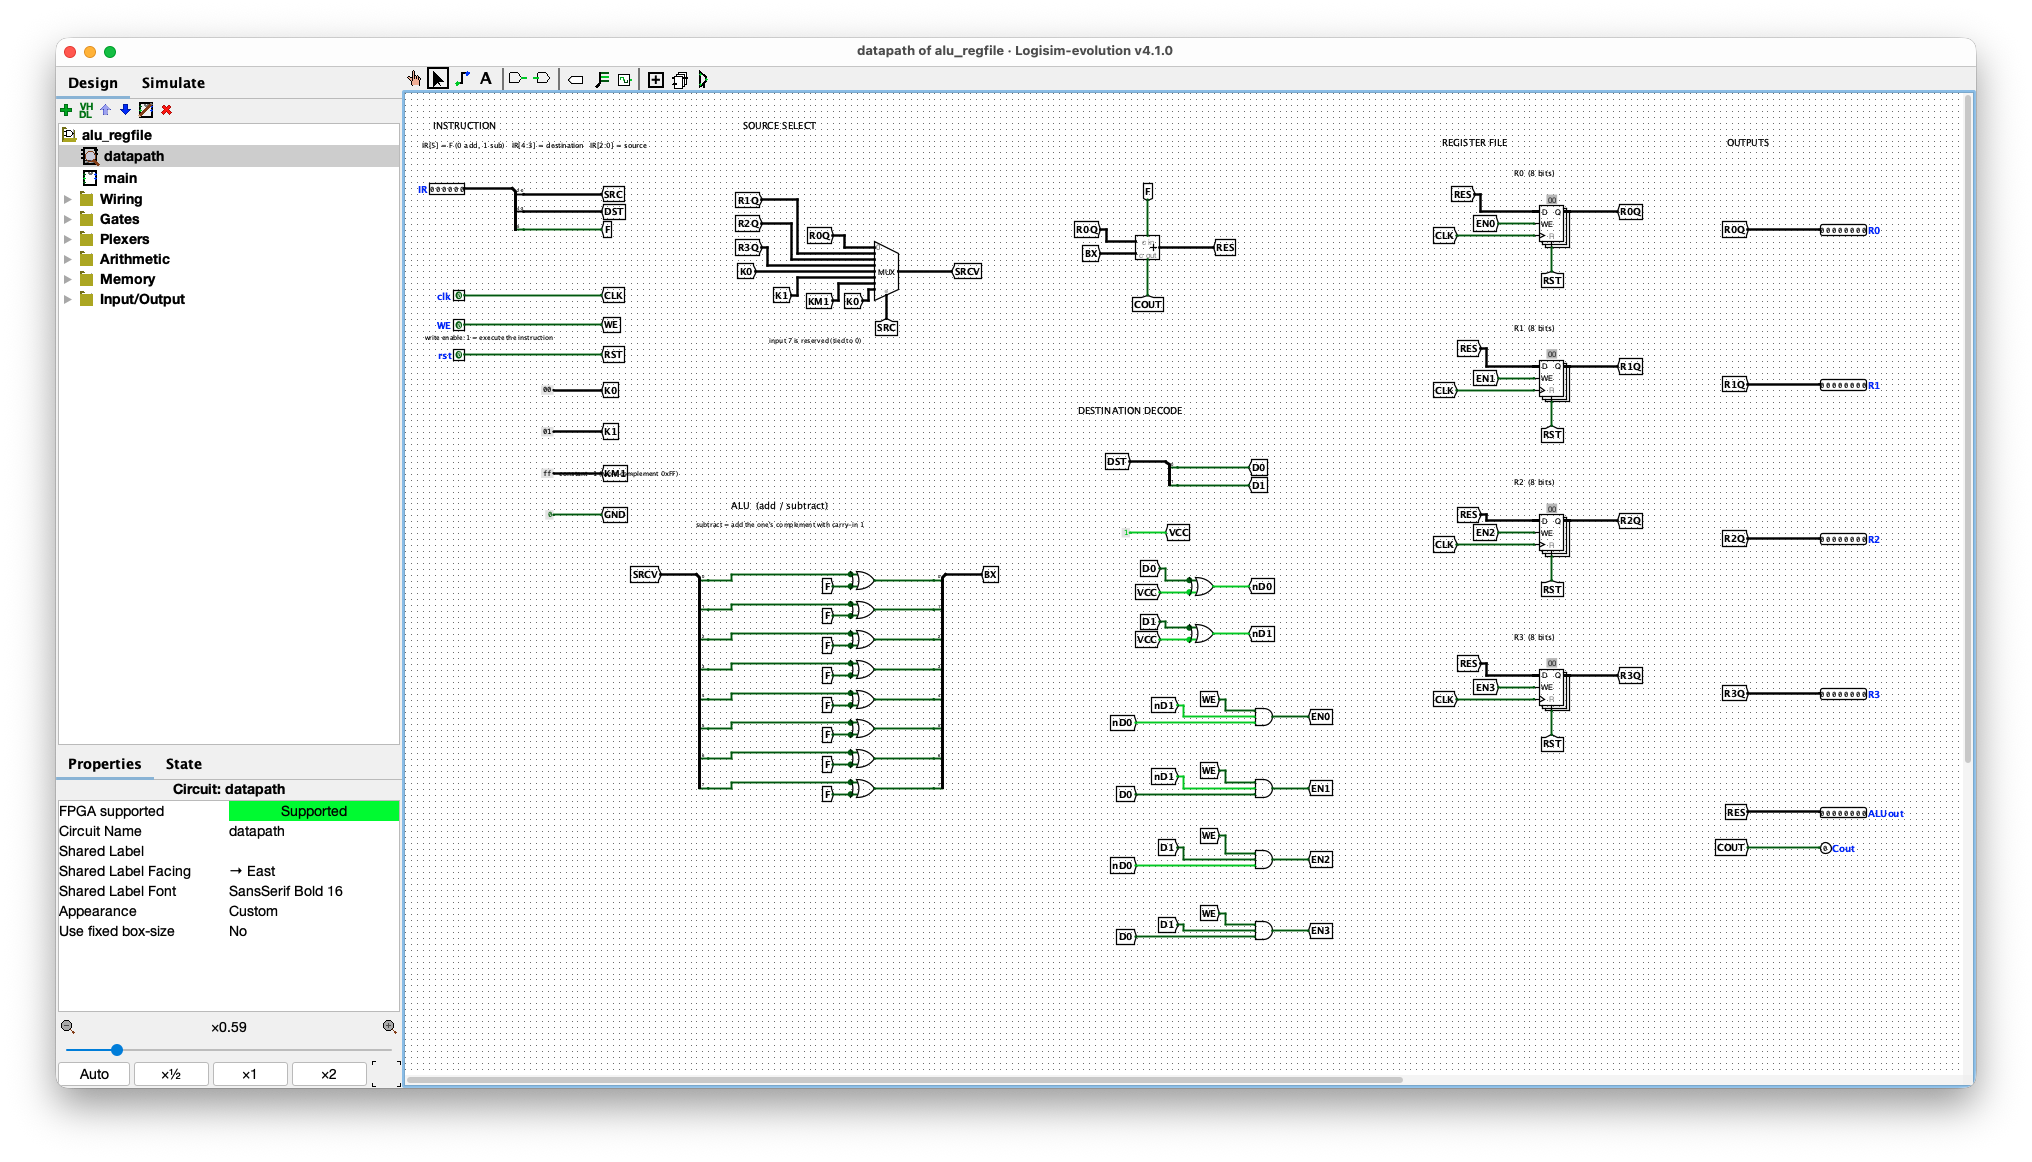
\includegraphics[width=1\textwidth]{figs/image2.png}
  \caption{نمای کلی مدار \lr{datapath}}
\end{figure}



% -------------------------- مدار main کامل ---------------------------
\begin{figure}[H]
  \centering
  
\includegraphics[width=1\textwidth]{figs/image.png}
  \caption{مدار \lr{main} با ورودی‌های مجزای فرمان و قطعه‌ی \lr{Clock}}
\end{figure}


نکته: در نوشتن این گزارش و تهیه‌ی جداول از هوش مصنوعی استفاده شده است.

\end{document}
